\section{The Sommelier System}\label{design}

\myparagraph{Data Cleanup}

The data source I have used for my project is the wines database belonging to Decanter.com\cite{DecanterCom}. The database contains nearly 40,000 professional ratings and tasting notes for wines from as far back as 1986, featuring vintages as far back as 1917.

The original database is highly inconsistent, displaying a mixture of design approaches and a variable quality of data. This is consistent with the fact that the database has been developed over a long period of time by a number of different developers with varying levels of skill, and that wine journalists making entries into the database have taken a number of idiosyncratic approaches to data entry.

Nevertheless I considered there to be a great deal of useful and interesting information in the database, with it to contain usable ratings and/or tastings for over 33,000 wines.

\begin{figure}[h!]
    \caption{Decanter.com Database}
    \centering
        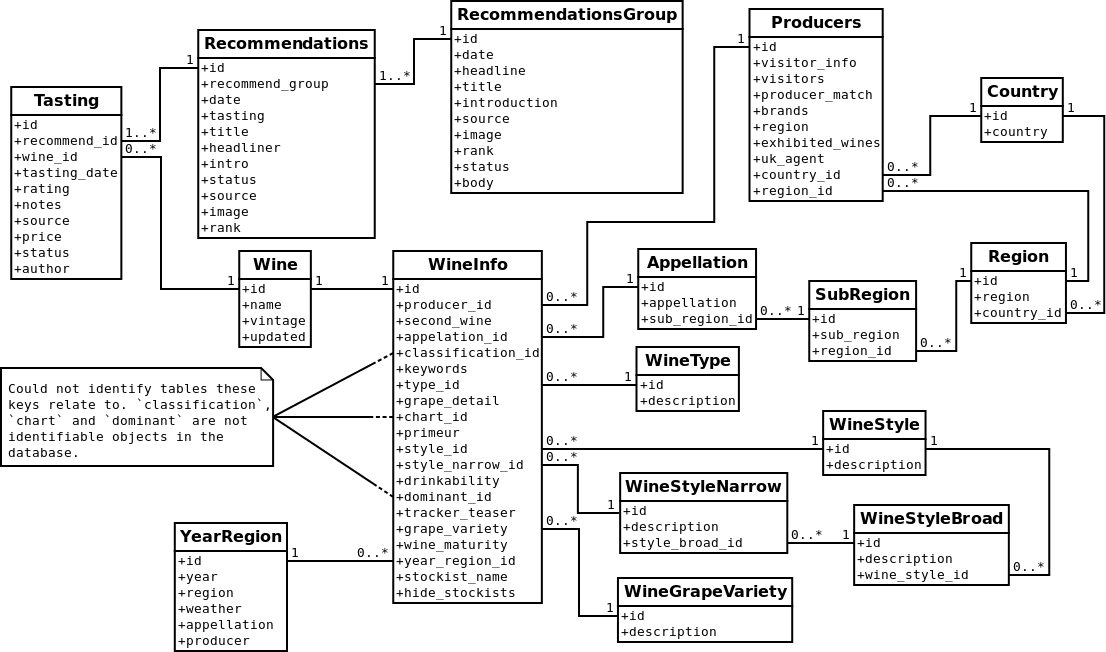
\includegraphics[width=14cm]{DecanterWineDB}
    \label{fig:decanterdb}
\end{figure}

The WineInfo table is a mixture of foreign keys joining to very small tables, such as WineInfo.type\_id joining to WineType.id where WineType is a table with only two attributes. This approach, stiving for a high degree of normalisation, contrasts with the fact that the same table also has the attribute second\_wine, as a string which only holds data in 450 of the 38762 entries in the table.

\myparagraph{Creating The Sommelier Dataset}

\begin{figure}[h!]
    \caption{Sommelier Database}
    \centering
        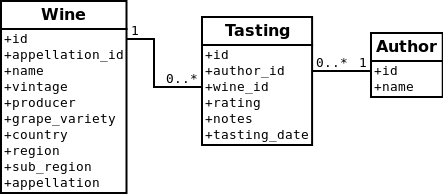
\includegraphics[width=10cm]{SommelierDBSimple}
    \label{fig:sommelierdb}
\end{figure}

For the new Sommelier database, Figure \ref{fig:sommelierdb}, I decided to denormalise [explanation/citation needed!] the wine data. This enables the data to be queried without joins, maximising the simplicity and execution speed of the queries [citation needed]. Denormalization makes data integrity difficult to maintain however, as there are potentially a large number of records to update for any change in a duplicated value. In this case an appellation or sub-region name changing might require thousands of records to be amended. Creating and editing wines is not a requirement of my system though, so for the purposes of this project the wine and tasting data is static and will not be subject to updates. For this reason the duplication of data within the Wine records is not problematic. In a real world setting this would need to be revisited.

Much of the data from the original database was disregarded entirely.

The tables WineStyleNarrow and WineStyleBroad contained generic text descriptions for wine (``rich and creamy'', ``crisp and tangy'' etc.). I initially considered this to have potential for migration into tag data which I could reuse as part of my filtering. Unfortunately less than 6435 of the records in WineInfo had non-null values for their style\_narrow\_id field, and only 3397 of these had corresponding records in the Tasting table. This figure was only around 10\% of the number of wines I expected the Sommelier database to contain so I decided that the WineStyle* tables were probably not worthwhile to migrate.

The WineType table was ignored because no wines corresponded to it; no WineInfo.type\_id record matched any WineType.id.

\myparagraph{The Author Problem}

The biggest shortcoming of the dataset is that the author of a tasting note is often not recorded. The number of wines with notes and known authors is only 1401, with there being 18 named authors on the system. 

Table \ref{table:authors} shows the distribution of tastings amongst authors, only 5 of which have tasted and rated more than 100 wines in the database.

\begin{table}[ht]
\caption{Authors of tasting notes and ratings}
\centering
\begin{tabular}{c c}
\\\hline\hline
Author               & Wines tasted, with notes and rating
\\\hline
Amy Wislocki         &            28 \\
Andrew Jefford       &           105 \\
Beverley Blanning MW &            13 \\
Carolyn Holmes       &             1 \\
Christelle Guibert   &           119 \\
Clive Coates MW      &             6 \\
David Peppercorn     &            44 \\
Gerald D Boyd        &             7 \\
Harriet Waugh        &           250 \\
James Lawther MW     &           226 \\
John Radford         &             2 \\
Josephine Butchart   &            24 \\
Norm Roby            &             4 \\
Rosemary George MW   &             6 \\
Serena Sutcliffe     &            31 \\
Stephen Brook        &            19 \\
Steven Spurrier      &           497 \\
\\\hline
\end{tabular}
\label{table:authors}
\end{table}

In some cases an author's initials or full name are recorded within the text of a tasting note. I decided that extracting and making use of these was impractical given the time constraints of this project.

DESCRIBE DATA SETS BEFORE AND AFTER

THE SOMMELIER DATASET

Having analysed the dataset and conceived an ideal schema, I needed to decide what the criteria to apply when extracting my new dataset from the source data.

Given that the purpose of the dataset is social recommendations, the first decision I made was to discard any wines without both tasting notes and a rating, whether.
